% Options for packages loaded elsewhere
\PassOptionsToPackage{unicode}{hyperref}
\PassOptionsToPackage{hyphens}{url}
%
\documentclass[
]{article}
\title{Testing out a 3-chapter dissertation as child documents}
\author{}
\date{\vspace{-2.5em}Last compiled 2022-02-20}

\usepackage{amsmath,amssymb}
\usepackage{lmodern}
\usepackage{iftex}
\ifPDFTeX
  \usepackage[T1]{fontenc}
  \usepackage[utf8]{inputenc}
  \usepackage{textcomp} % provide euro and other symbols
\else % if luatex or xetex
  \usepackage{unicode-math}
  \defaultfontfeatures{Scale=MatchLowercase}
  \defaultfontfeatures[\rmfamily]{Ligatures=TeX,Scale=1}
  \setmainfont[]{Roboto}
\fi
% Use upquote if available, for straight quotes in verbatim environments
\IfFileExists{upquote.sty}{\usepackage{upquote}}{}
\IfFileExists{microtype.sty}{% use microtype if available
  \usepackage[]{microtype}
  \UseMicrotypeSet[protrusion]{basicmath} % disable protrusion for tt fonts
}{}
\makeatletter
\@ifundefined{KOMAClassName}{% if non-KOMA class
  \IfFileExists{parskip.sty}{%
    \usepackage{parskip}
  }{% else
    \setlength{\parindent}{0pt}
    \setlength{\parskip}{6pt plus 2pt minus 1pt}}
}{% if KOMA class
  \KOMAoptions{parskip=half}}
\makeatother
\usepackage{xcolor}
\IfFileExists{xurl.sty}{\usepackage{xurl}}{} % add URL line breaks if available
\IfFileExists{bookmark.sty}{\usepackage{bookmark}}{\usepackage{hyperref}}
\hypersetup{
  pdftitle={Testing out a 3-chapter dissertation as child documents},
  hidelinks,
  pdfcreator={LaTeX via pandoc}}
\urlstyle{same} % disable monospaced font for URLs
\usepackage[margin=1in]{geometry}
\usepackage{longtable,booktabs,array}
\usepackage{calc} % for calculating minipage widths
% Correct order of tables after \paragraph or \subparagraph
\usepackage{etoolbox}
\makeatletter
\patchcmd\longtable{\par}{\if@noskipsec\mbox{}\fi\par}{}{}
\makeatother
% Allow footnotes in longtable head/foot
\IfFileExists{footnotehyper.sty}{\usepackage{footnotehyper}}{\usepackage{footnote}}
\makesavenoteenv{longtable}
\usepackage{graphicx}
\makeatletter
\def\maxwidth{\ifdim\Gin@nat@width>\linewidth\linewidth\else\Gin@nat@width\fi}
\def\maxheight{\ifdim\Gin@nat@height>\textheight\textheight\else\Gin@nat@height\fi}
\makeatother
% Scale images if necessary, so that they will not overflow the page
% margins by default, and it is still possible to overwrite the defaults
% using explicit options in \includegraphics[width, height, ...]{}
\setkeys{Gin}{width=\maxwidth,height=\maxheight,keepaspectratio}
% Set default figure placement to htbp
\makeatletter
\def\fps@figure{htbp}
\makeatother
\setlength{\emergencystretch}{3em} % prevent overfull lines
\providecommand{\tightlist}{%
  \setlength{\itemsep}{0pt}\setlength{\parskip}{0pt}}
\setcounter{secnumdepth}{5}
\newlength{\cslhangindent}
\setlength{\cslhangindent}{1.5em}
\newlength{\csllabelwidth}
\setlength{\csllabelwidth}{3em}
\newlength{\cslentryspacingunit} % times entry-spacing
\setlength{\cslentryspacingunit}{\parskip}
\newenvironment{CSLReferences}[2] % #1 hanging-ident, #2 entry spacing
 {% don't indent paragraphs
  \setlength{\parindent}{0pt}
  % turn on hanging indent if param 1 is 1
  \ifodd #1
  \let\oldpar\par
  \def\par{\hangindent=\cslhangindent\oldpar}
  \fi
  % set entry spacing
  \setlength{\parskip}{#2\cslentryspacingunit}
 }%
 {}
\usepackage{calc}
\newcommand{\CSLBlock}[1]{#1\hfill\break}
\newcommand{\CSLLeftMargin}[1]{\parbox[t]{\csllabelwidth}{#1}}
\newcommand{\CSLRightInline}[1]{\parbox[t]{\linewidth - \csllabelwidth}{#1}\break}
\newcommand{\CSLIndent}[1]{\hspace{\cslhangindent}#1}
\usepackage{booktabs}
\usepackage{longtable}
\usepackage{array}
\usepackage{multirow}
\usepackage{wrapfig}
\usepackage{float}
\usepackage{colortbl}
\usepackage{pdflscape}
\usepackage{tabu}
\usepackage{threeparttable}
\usepackage{threeparttablex}
\usepackage[normalem]{ulem}
\usepackage{makecell}
\usepackage{xcolor}
\ifLuaTeX
  \usepackage{selnolig}  % disable illegal ligatures
\fi

\begin{document}
\maketitle

{
\setcounter{tocdepth}{2}
\tableofcontents
}
\hypertarget{the-first-chapter}{%
\section{The first chapter}\label{the-first-chapter}}

\hypertarget{introduction}{%
\subsection{Introduction}\label{introduction}}

Some literature review.

A reference is (Atterberg 1974).

\hypertarget{materials-and-methods}{%
\subsection{Materials and Methods}\label{materials-and-methods}}

Blah blah blah

See Table \ref{tab:ch-1-table}.

\begin{table}

\caption{\label{tab:ch-1-table}The mtcars dataset.}
\centering
\begin{tabular}[t]{l|r|r|r|r|r|r|r|r|r|r|r}
\hline
  & mpg & cyl & disp & hp & drat & wt & qsec & vs & am & gear & carb\\
\hline
Mazda RX4 & 21.0 & 6 & 160.0 & 110 & 3.90 & 2.620 & 16.46 & 0 & 1 & 4 & 4\\
\hline
Mazda RX4 Wag & 21.0 & 6 & 160.0 & 110 & 3.90 & 2.875 & 17.02 & 0 & 1 & 4 & 4\\
\hline
Datsun 710 & 22.8 & 4 & 108.0 & 93 & 3.85 & 2.320 & 18.61 & 1 & 1 & 4 & 1\\
\hline
Hornet 4 Drive & 21.4 & 6 & 258.0 & 110 & 3.08 & 3.215 & 19.44 & 1 & 0 & 3 & 1\\
\hline
Hornet Sportabout & 18.7 & 8 & 360.0 & 175 & 3.15 & 3.440 & 17.02 & 0 & 0 & 3 & 2\\
\hline
Valiant & 18.1 & 6 & 225.0 & 105 & 2.76 & 3.460 & 20.22 & 1 & 0 & 3 & 1\\
\hline
Duster 360 & 14.3 & 8 & 360.0 & 245 & 3.21 & 3.570 & 15.84 & 0 & 0 & 3 & 4\\
\hline
Merc 240D & 24.4 & 4 & 146.7 & 62 & 3.69 & 3.190 & 20.00 & 1 & 0 & 4 & 2\\
\hline
Merc 230 & 22.8 & 4 & 140.8 & 95 & 3.92 & 3.150 & 22.90 & 1 & 0 & 4 & 2\\
\hline
Merc 280 & 19.2 & 6 & 167.6 & 123 & 3.92 & 3.440 & 18.30 & 1 & 0 & 4 & 4\\
\hline
Merc 280C & 17.8 & 6 & 167.6 & 123 & 3.92 & 3.440 & 18.90 & 1 & 0 & 4 & 4\\
\hline
Merc 450SE & 16.4 & 8 & 275.8 & 180 & 3.07 & 4.070 & 17.40 & 0 & 0 & 3 & 3\\
\hline
Merc 450SL & 17.3 & 8 & 275.8 & 180 & 3.07 & 3.730 & 17.60 & 0 & 0 & 3 & 3\\
\hline
Merc 450SLC & 15.2 & 8 & 275.8 & 180 & 3.07 & 3.780 & 18.00 & 0 & 0 & 3 & 3\\
\hline
Cadillac Fleetwood & 10.4 & 8 & 472.0 & 205 & 2.93 & 5.250 & 17.98 & 0 & 0 & 3 & 4\\
\hline
Lincoln Continental & 10.4 & 8 & 460.0 & 215 & 3.00 & 5.424 & 17.82 & 0 & 0 & 3 & 4\\
\hline
Chrysler Imperial & 14.7 & 8 & 440.0 & 230 & 3.23 & 5.345 & 17.42 & 0 & 0 & 3 & 4\\
\hline
Fiat 128 & 32.4 & 4 & 78.7 & 66 & 4.08 & 2.200 & 19.47 & 1 & 1 & 4 & 1\\
\hline
Honda Civic & 30.4 & 4 & 75.7 & 52 & 4.93 & 1.615 & 18.52 & 1 & 1 & 4 & 2\\
\hline
Toyota Corolla & 33.9 & 4 & 71.1 & 65 & 4.22 & 1.835 & 19.90 & 1 & 1 & 4 & 1\\
\hline
Toyota Corona & 21.5 & 4 & 120.1 & 97 & 3.70 & 2.465 & 20.01 & 1 & 0 & 3 & 1\\
\hline
Dodge Challenger & 15.5 & 8 & 318.0 & 150 & 2.76 & 3.520 & 16.87 & 0 & 0 & 3 & 2\\
\hline
AMC Javelin & 15.2 & 8 & 304.0 & 150 & 3.15 & 3.435 & 17.30 & 0 & 0 & 3 & 2\\
\hline
Camaro Z28 & 13.3 & 8 & 350.0 & 245 & 3.73 & 3.840 & 15.41 & 0 & 0 & 3 & 4\\
\hline
Pontiac Firebird & 19.2 & 8 & 400.0 & 175 & 3.08 & 3.845 & 17.05 & 0 & 0 & 3 & 2\\
\hline
Fiat X1-9 & 27.3 & 4 & 79.0 & 66 & 4.08 & 1.935 & 18.90 & 1 & 1 & 4 & 1\\
\hline
Porsche 914-2 & 26.0 & 4 & 120.3 & 91 & 4.43 & 2.140 & 16.70 & 0 & 1 & 5 & 2\\
\hline
Lotus Europa & 30.4 & 4 & 95.1 & 113 & 3.77 & 1.513 & 16.90 & 1 & 1 & 5 & 2\\
\hline
Ford Pantera L & 15.8 & 8 & 351.0 & 264 & 4.22 & 3.170 & 14.50 & 0 & 1 & 5 & 4\\
\hline
Ferrari Dino & 19.7 & 6 & 145.0 & 175 & 3.62 & 2.770 & 15.50 & 0 & 1 & 5 & 6\\
\hline
Maserati Bora & 15.0 & 8 & 301.0 & 335 & 3.54 & 3.570 & 14.60 & 0 & 1 & 5 & 8\\
\hline
Volvo 142E & 21.4 & 4 & 121.0 & 109 & 4.11 & 2.780 & 18.60 & 1 & 1 & 4 & 2\\
\hline
\end{tabular}
\end{table}

\hypertarget{results-and-discussion}{%
\subsection{Results and Discussion}\label{results-and-discussion}}

Some results. See Figure \ref{fig:mt-cars-plot}

\begin{figure}
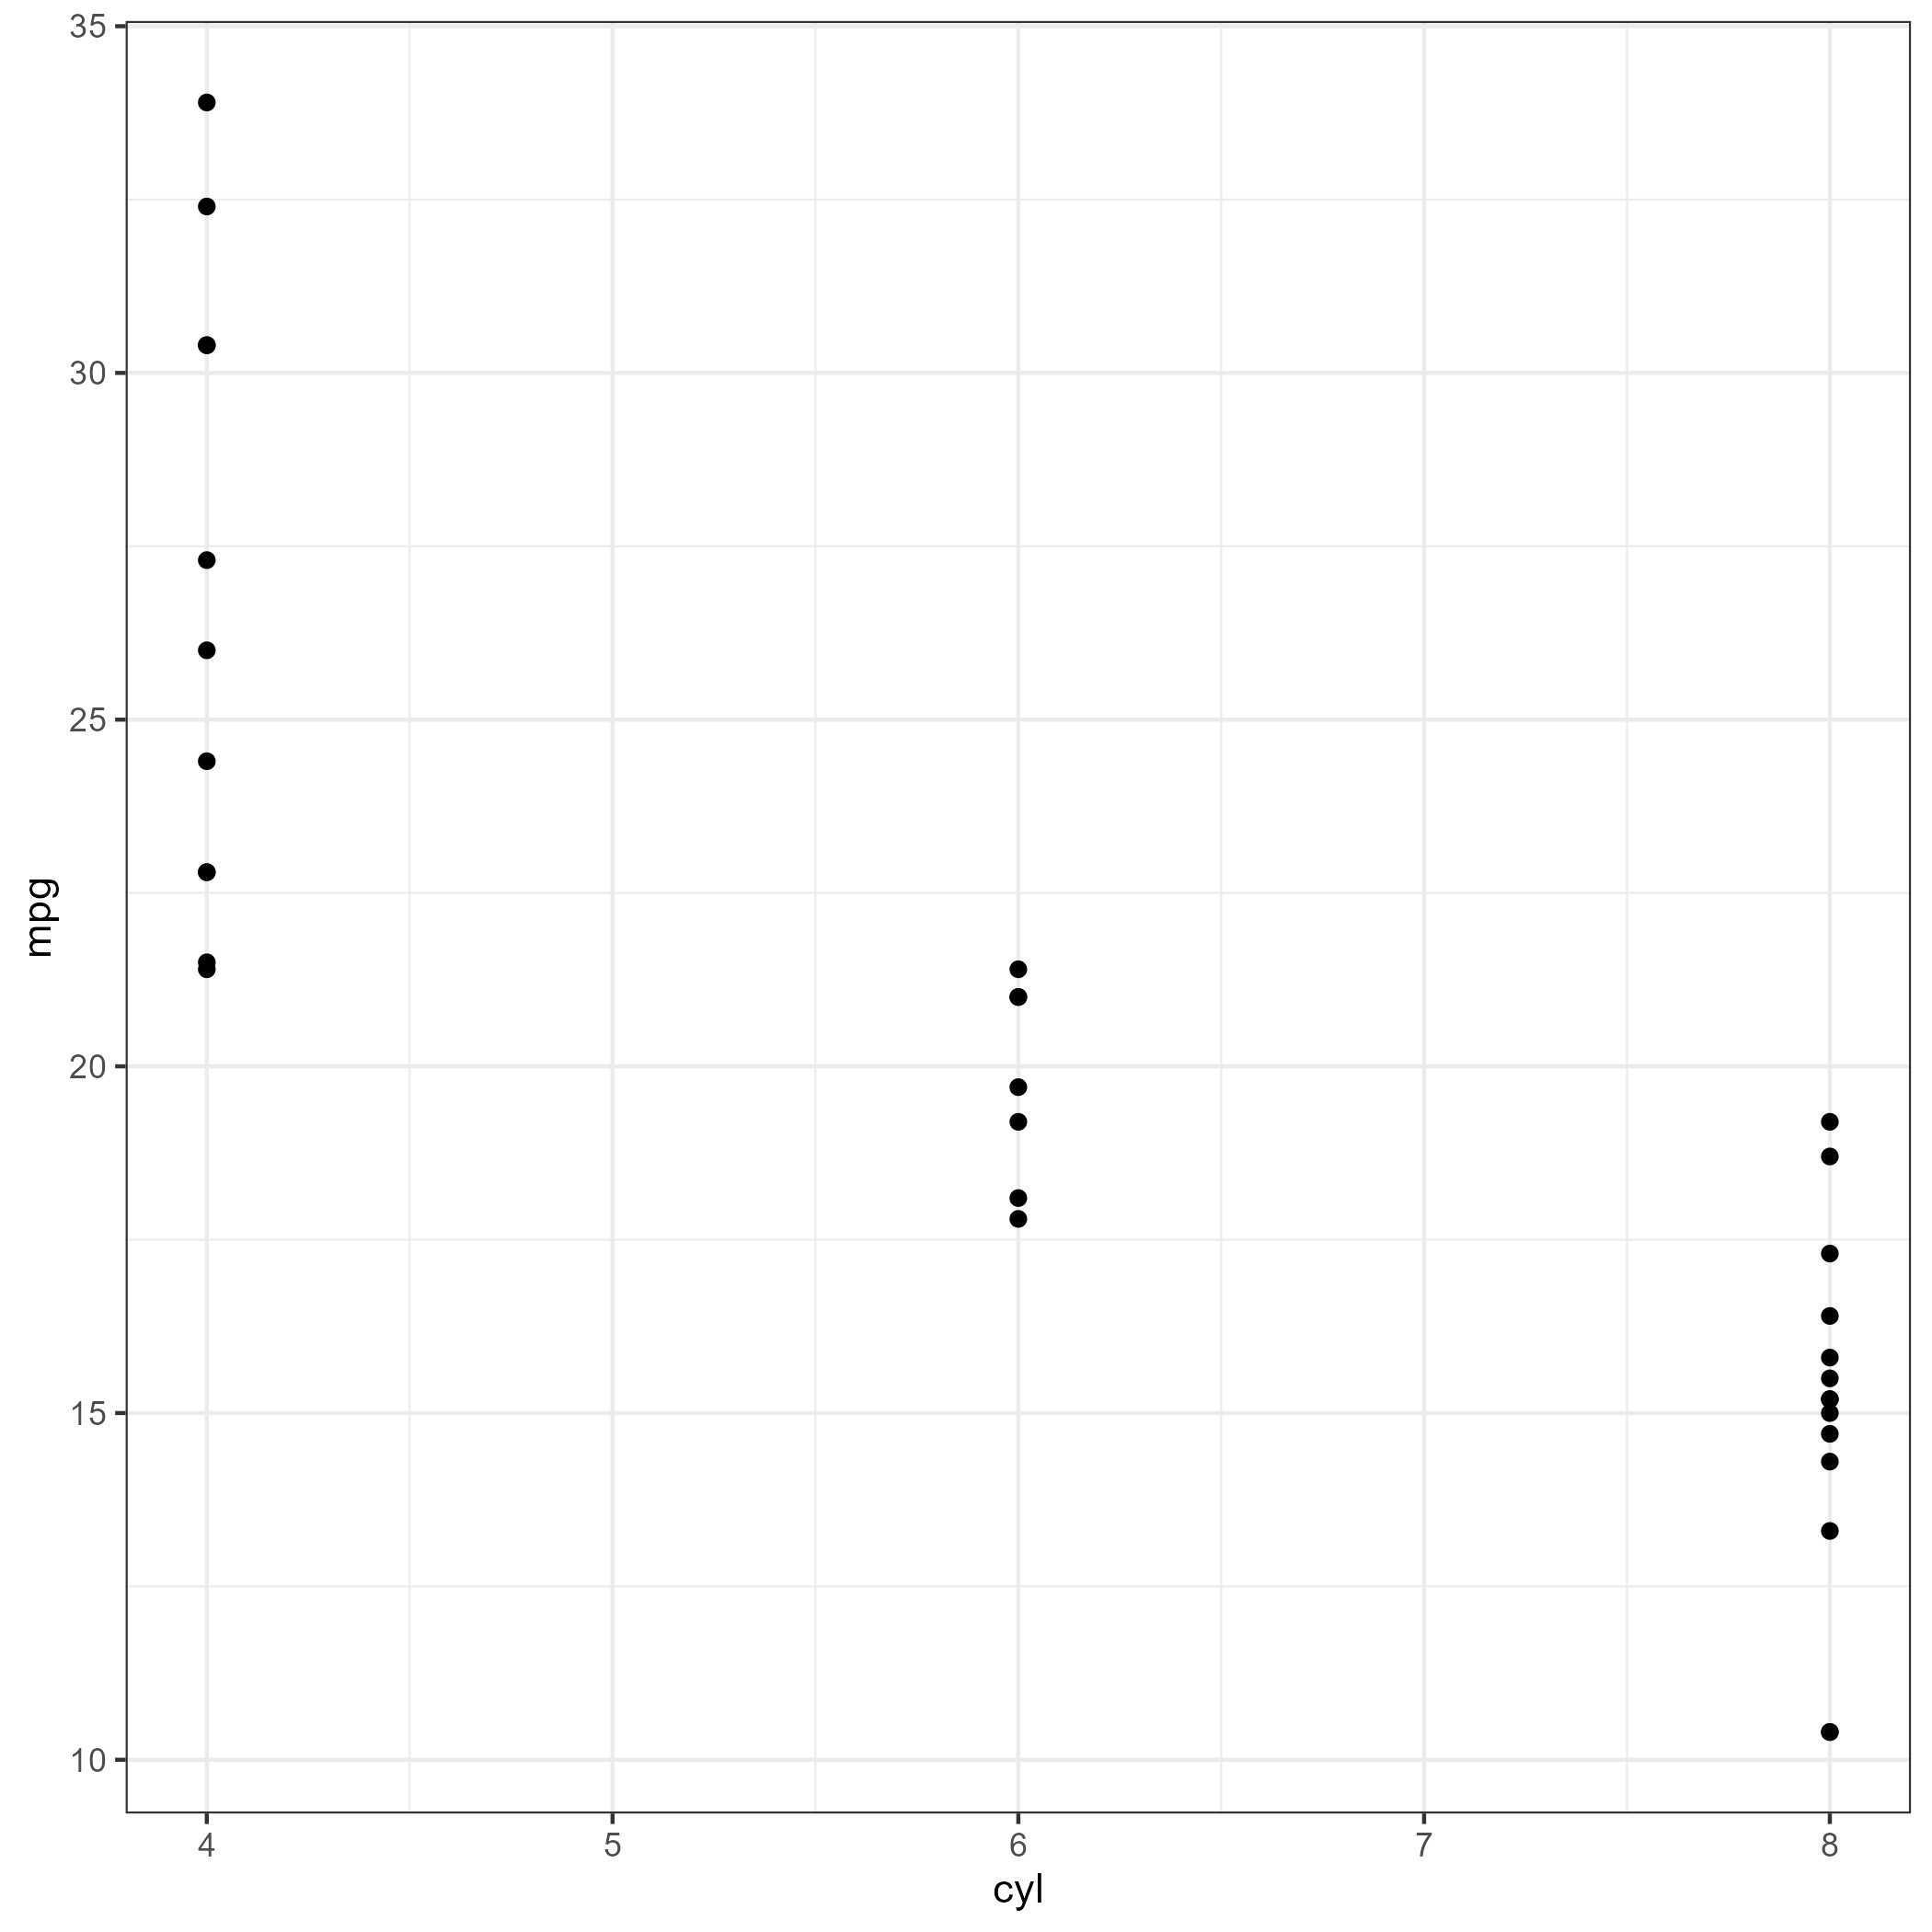
\includegraphics[width=29.17in]{E:/OneDrive - The Pennsylvania State University/PSU2019-present/A_inf_soils_PhD/drafts/dissertation-makefile-test/chapter-1/mt-cars-plot} \caption{A plot from the mtcars dataset.}\label{fig:mt-cars-plot}
\end{figure}

\hypertarget{conclusions}{%
\subsection{Conclusions}\label{conclusions}}

A conclusion.

\hypertarget{references}{%
\subsection{References}\label{references}}

\clearpage

\hypertarget{the-second-chapter}{%
\section{The second chapter}\label{the-second-chapter}}

\hypertarget{introduction-1}{%
\subsection{Introduction}\label{introduction-1}}

Some literature review.

A reference is (Barnes 2013).

\hypertarget{materials-and-methods-1}{%
\subsection{Materials and Methods}\label{materials-and-methods-1}}

Blah blah blah

See Table \ref{tab:ch-2-table}.

\begin{table}

\caption{\label{tab:ch-2-table}A table regarding storms.}
\centering
\begin{tabular}[t]{l|r|r|r|r|r|r|l|l|r|r|r|r}
\hline
name & year & month & day & hour & lat & long & status & category & wind & pressure & ts\_diameter & hu\_diameter\\
\hline
Amy & 1975 & 6 & 27 & 0 & 27.5 & -79.0 & tropical depression & -1 & 25 & 1013 & NA & NA\\
\hline
Amy & 1975 & 6 & 27 & 6 & 28.5 & -79.0 & tropical depression & -1 & 25 & 1013 & NA & NA\\
\hline
Amy & 1975 & 6 & 27 & 12 & 29.5 & -79.0 & tropical depression & -1 & 25 & 1013 & NA & NA\\
\hline
Amy & 1975 & 6 & 27 & 18 & 30.5 & -79.0 & tropical depression & -1 & 25 & 1013 & NA & NA\\
\hline
Amy & 1975 & 6 & 28 & 0 & 31.5 & -78.8 & tropical depression & -1 & 25 & 1012 & NA & NA\\
\hline
Amy & 1975 & 6 & 28 & 6 & 32.4 & -78.7 & tropical depression & -1 & 25 & 1012 & NA & NA\\
\hline
\end{tabular}
\end{table}

\hypertarget{results-and-discussion-1}{%
\subsection{Results and Discussion}\label{results-and-discussion-1}}

Some results. See Figure \ref{fig:storms-plot}

\begin{figure}
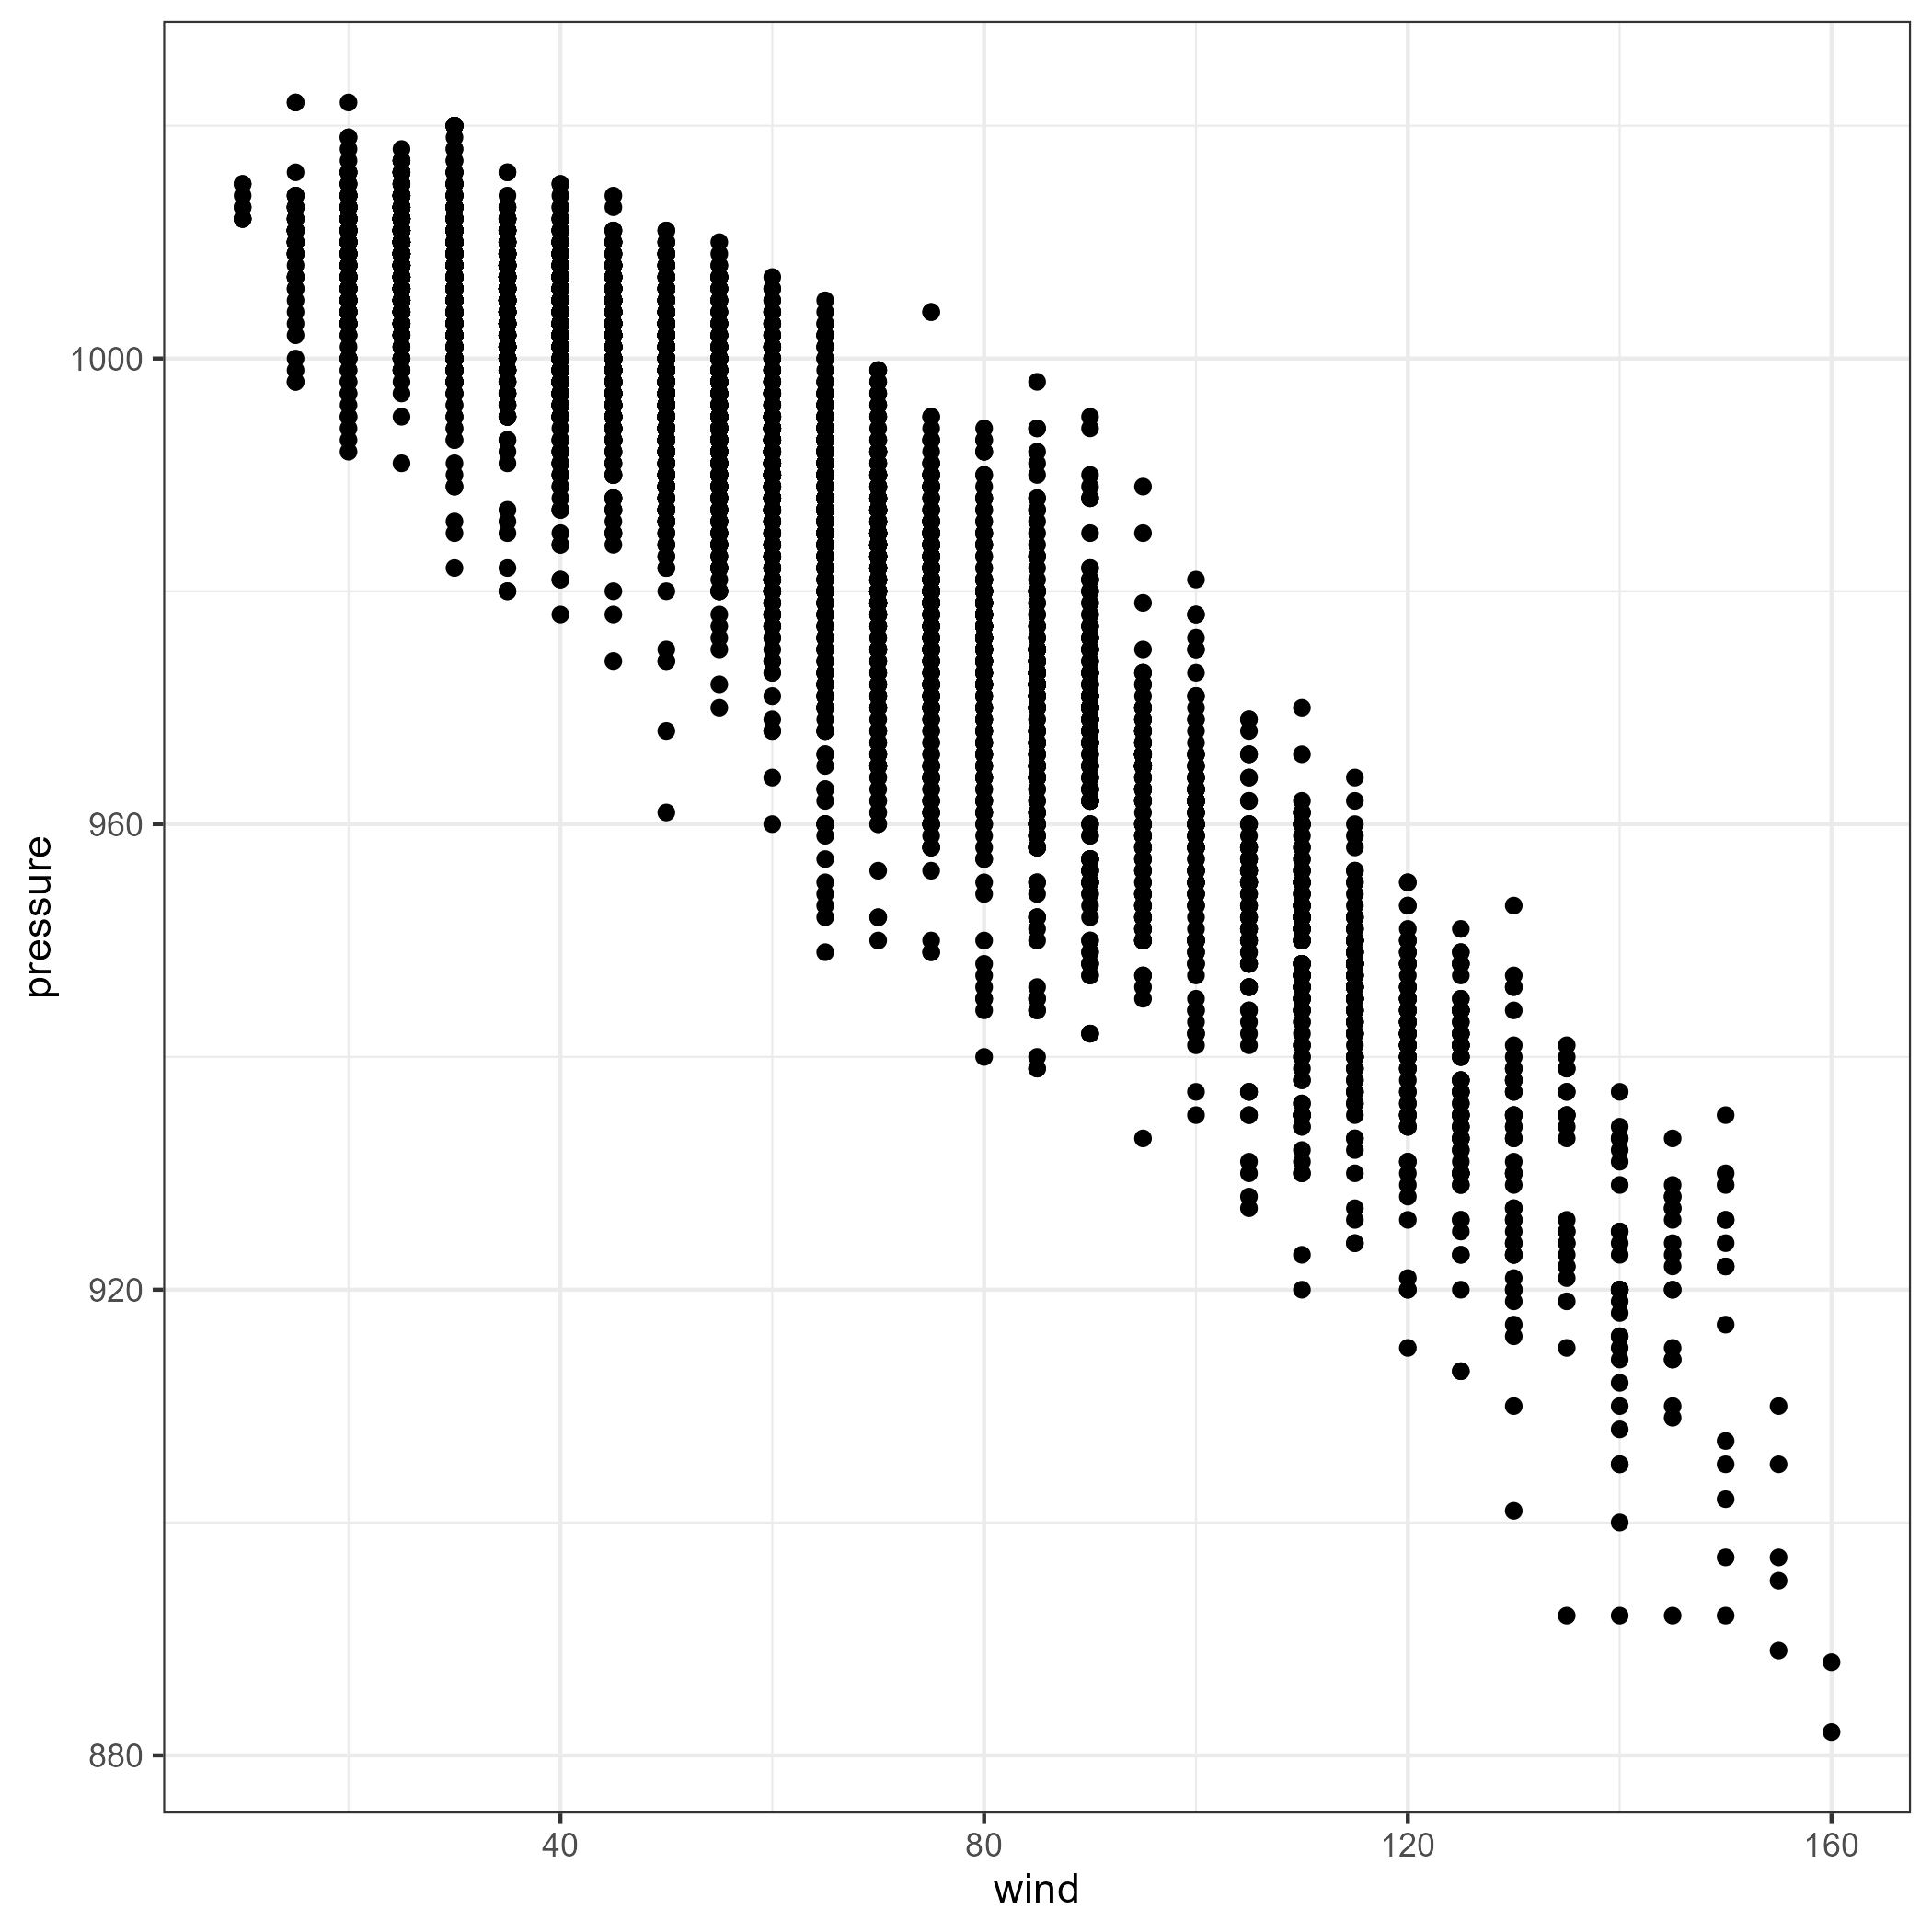
\includegraphics[width=29.17in]{E:/OneDrive - The Pennsylvania State University/PSU2019-present/A_inf_soils_PhD/drafts/dissertation-makefile-test/chapter-2/storms-plot} \caption{A plot from the storms dataset.}\label{fig:storms-plot}
\end{figure}

\hypertarget{conclusions-1}{%
\subsection{Conclusions}\label{conclusions-1}}

A conclusion.

\hypertarget{references-1}{%
\subsection{References}\label{references-1}}

\clearpage

\hypertarget{the-third-chapter}{%
\section{The third chapter}\label{the-third-chapter}}

\hypertarget{introduction-2}{%
\subsection{Introduction}\label{introduction-2}}

Baseball infields must provide stable footing and predictable ball response.

A reference is (Holtz, Kovacs, and Sheahan 2010).

\hypertarget{materials-and-methods-2}{%
\subsection{Materials and Methods}\label{materials-and-methods-2}}

Blah blah blah

See Table \ref{tab:ch-3-table}.

\begin{table}

\caption{\label{tab:ch-3-table}Air quality data.}
\centering
\begin{tabular}[t]{r|r|r|r|r|r}
\hline
Ozone & Solar.R & Wind & Temp & Month & Day\\
\hline
41 & 190 & 7.4 & 67 & 5 & 1\\
\hline
36 & 118 & 8.0 & 72 & 5 & 2\\
\hline
12 & 149 & 12.6 & 74 & 5 & 3\\
\hline
18 & 313 & 11.5 & 62 & 5 & 4\\
\hline
NA & NA & 14.3 & 56 & 5 & 5\\
\hline
28 & NA & 14.9 & 66 & 5 & 6\\
\hline
\end{tabular}
\end{table}

\hypertarget{results-and-discussion-2}{%
\subsection{Results and Discussion}\label{results-and-discussion-2}}

Some results. See Figure \ref{fig:airquality-plot}

\begin{figure}
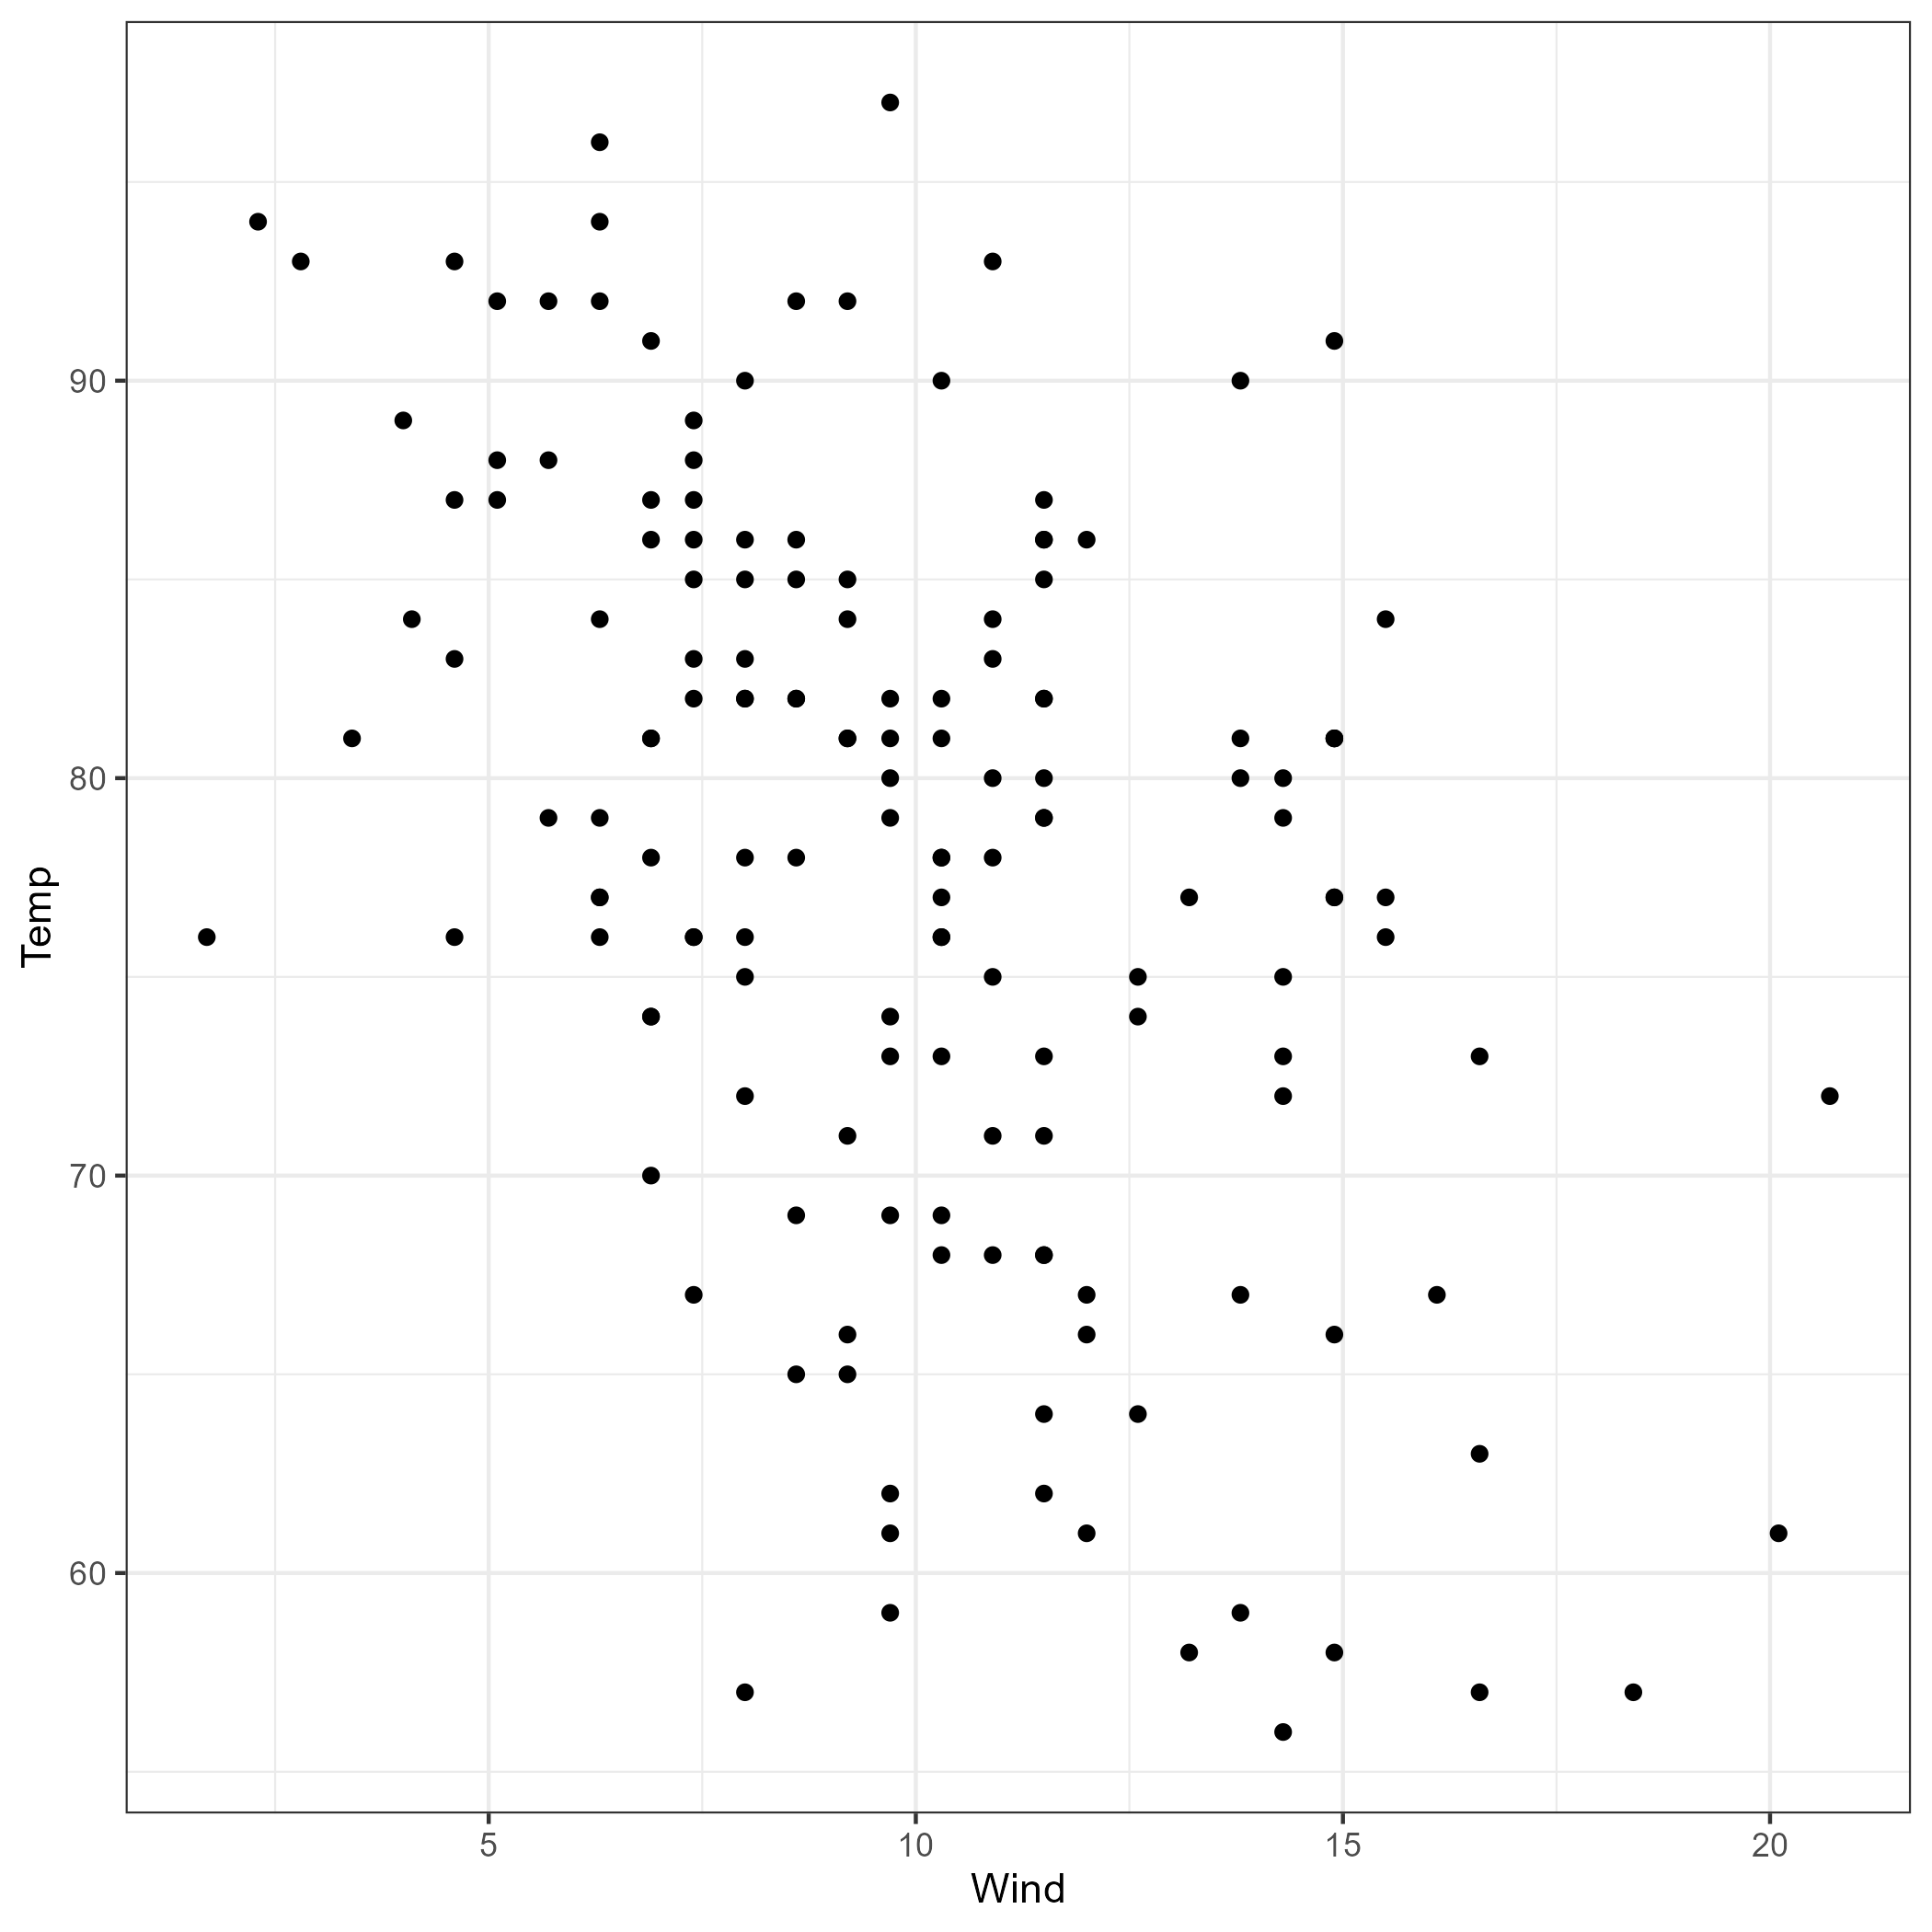
\includegraphics[width=29.17in]{E:/OneDrive - The Pennsylvania State University/PSU2019-present/A_inf_soils_PhD/drafts/dissertation-makefile-test/chapter-3/airquality-plot} \caption{A plot from the airquality dataset.}\label{fig:airquality-plot}
\end{figure}

\hypertarget{conclusions-2}{%
\subsection{Conclusions}\label{conclusions-2}}

A conclusion.

\hypertarget{references-2}{%
\subsection*{References}\label{references-2}}
\addcontentsline{toc}{subsection}{References}

\hypertarget{refs}{}
\begin{CSLReferences}{1}{0}
\leavevmode\vadjust pre{\hypertarget{ref-Atterberg1974}{}}%
Atterberg, Albert. 1974. {``Plasticity of Clays.''} {Hanover, NJ}: {Cold Regions Research Lab}.

\leavevmode\vadjust pre{\hypertarget{ref-Barnes2013}{}}%
Barnes, Graham Edward. 2013. {``The {Plastic Limit} and {Workability} of {Soils}.''} {University of Manchester}. \url{https://www.escholar.manchester.ac.uk/api/datastream?publicationPid=uk-ac-man-scw:212752\&datastreamId=FULL-TEXT.PDF}.

\leavevmode\vadjust pre{\hypertarget{ref-Holtz2010}{}}%
Holtz, Robert D., William D. Kovacs, and Thomas C. Sheahan. 2010. \emph{An {Introduction} to {Geotechnical Engineering}}. {New York, NY}: {Pearson}.

\end{CSLReferences}

\end{document}
